\subsection{Experiência 2}

Esta experiência teve como objetivo configurar duas VLAN's, bem como entender como funcionam domínios de broadcast.

\begin{figure}[!h]
\centering
  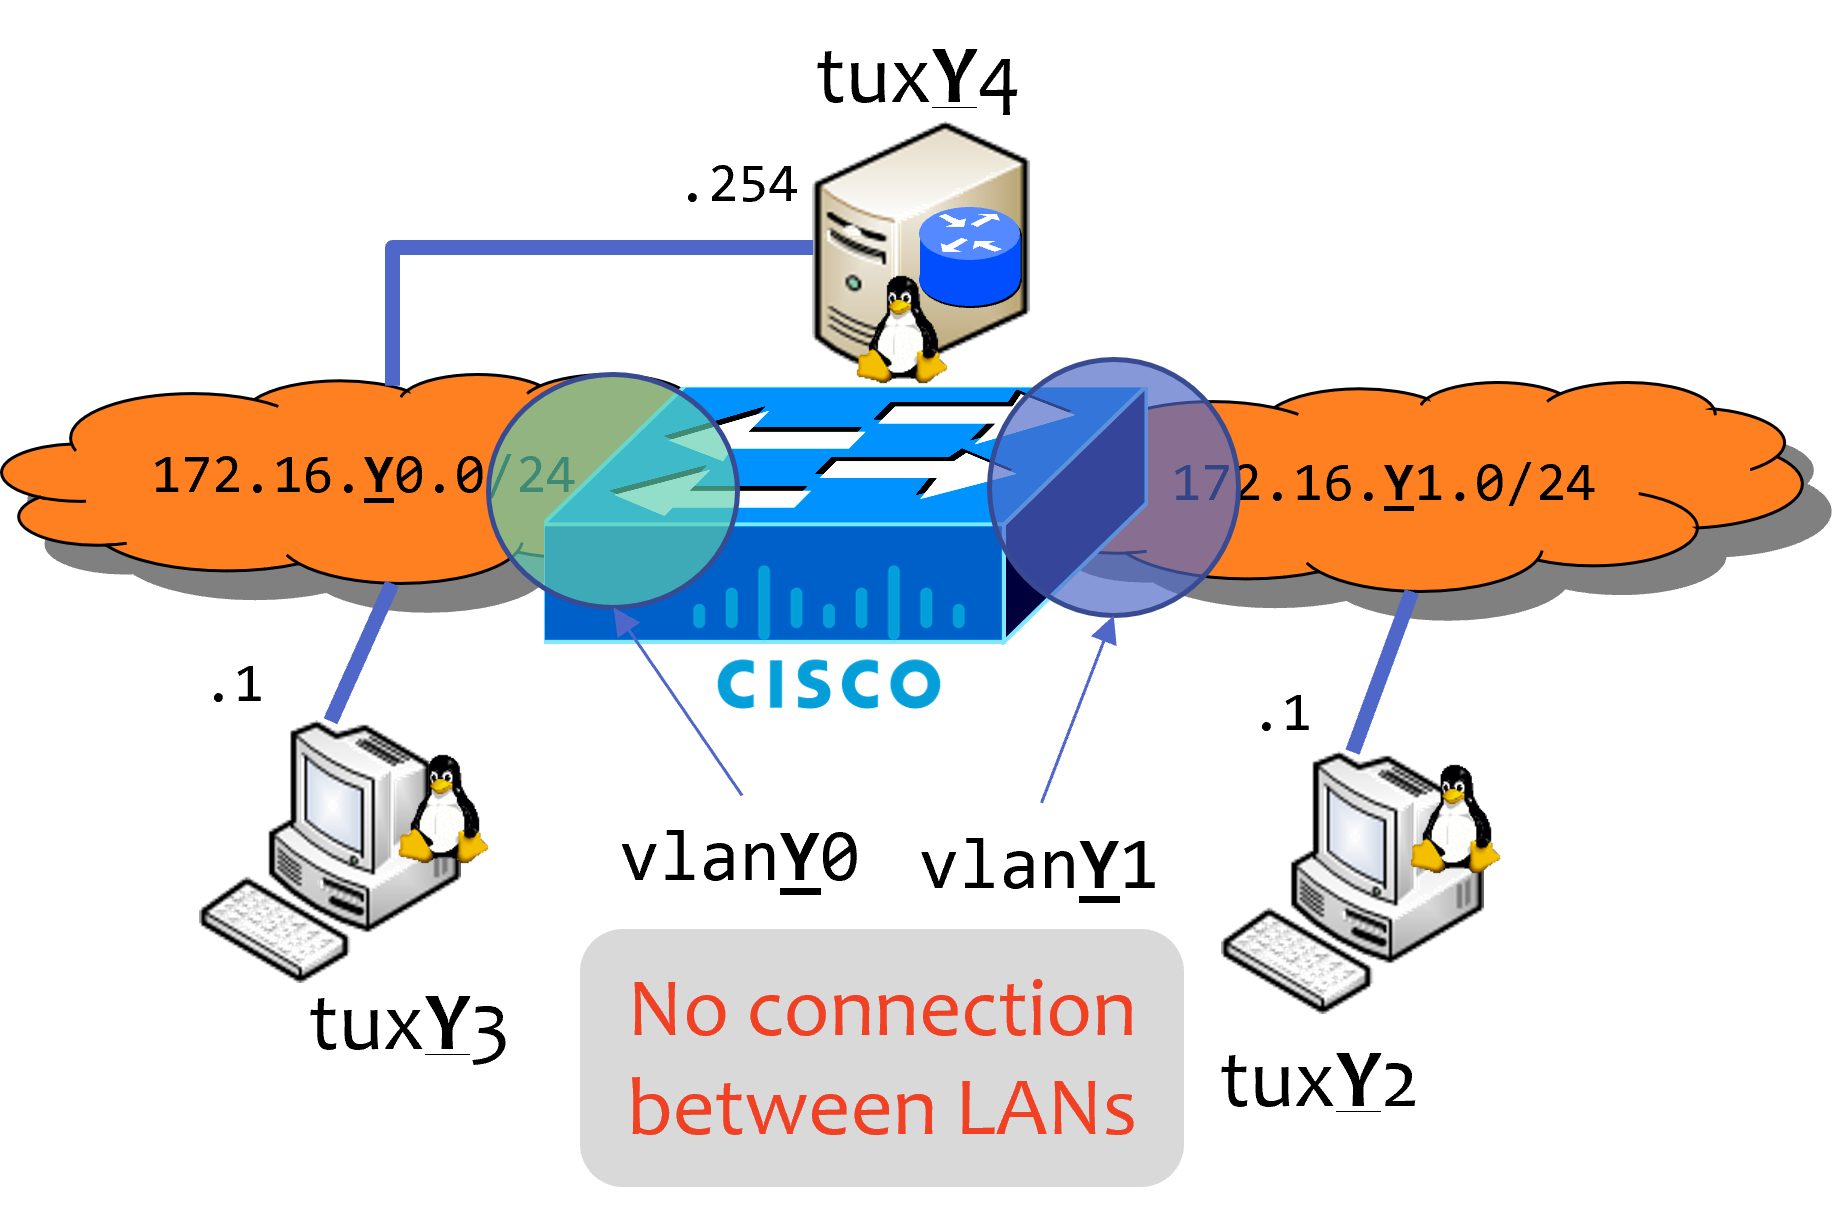
\includegraphics[width=.4\linewidth]{img/net-vlans.png}
  \caption{Estrutura da rede}
\end{figure}

\subsubsection{Questões}
\paragraph{Como configurar a vlan50}
Primeiro conecta-se a interface eht0 do tux53 à conexão correspondente à porta 1 do switch e o a interface eth0 do tux54 à conexão correspondente à porta 2. Em seguida configuramos os endereços IP de ambas as interfaces para que correspondam à especificação


\begin{center}
\begin{tabular}{ c c c }
    \textbf{Máquina} & \textbf{Interface} & \textbf{Endereço IP} \\ \hline 
    Tux53 & eth0 & 172.16.50.1 \\  
    Tux54 & eth0 & 172.16.50.254    
\end{tabular}
\end{center}


Em seguida criamos conectamos a porta série do Tux53 à porta série do switch e configuramos a VLAN50 com as portas 1 e 2 associadas à VLAN pois são as portas a que estão conectados os Tux53 e Tux54.

\paragraph{Quantos dominios de broadcast há? Como o podemos cocluir tendo por base os logs?}

Podemos concluir que há dois domínios de Broadcast. Um deles é na vlan50, uma vez que, os pacotes do ping do tux3 (172.16.50.1) atingem o tux4 (172.16.50.254), mas não atingem tux2(172.16.51.1) como se pode ver nas figuras (Figure 10 e Figure 12). O outro é na vlan51, no entanto, não há qualquer prova de Broadcast porque o tux2 se encontra isolado na vlan referida havendo apenas registo dos pacotes a saírem da origem como se pode ver na figura. (Figure 14)